%%%%%%%%%%%%%%%%%%%%%%%%%%%%%%%%%%%%%%%%%
% Short Sectioned Assignment
% LaTeX Template
% Version 1.0 (5/5/12)
%
% This template has been downloaded from:
% http://www.LaTeXTemplates.com
%
% Original author:
% Frits Wenneker (http://www.howtotex.com)
%
% License:
% CC BY-NC-SA 3.0 (http://creativecommons.org/licenses/by-nc-sa/3.0/)
%
%%%%%%%%%%%%%%%%%%%%%%%%%%%%%%%%%%%%%%%%%

%----------------------------------------------------------------------------------------
%	PACKAGES AND OTHER DOCUMENT CONFIGURATIONS
%----------------------------------------------------------------------------------------

\documentclass[paper=a4, fontsize=11pt]{scrartcl} % A4 paper and 11pt font size

\usepackage[T1]{fontenc} % Use 8-bit encoding that has 256 glyphs
\usepackage{fourier} % Use the Adobe Utopia font for the document - comment this line to return to the LaTeX default
\usepackage[english]{babel} % English language/hyphenation

\usepackage{lipsum} % Used for inserting dummy 'Lorem ipsum' text into the template

\usepackage{sectsty} % Allows customizing section commands
\allsectionsfont{ \normalfont\scshape} % Make all sections centered, the default font and small caps
\usepackage{cite}
\usepackage{listings}

%%%%%---------------------------%%%%%%%%%%%
\usepackage{fancybox}
\usepackage{graphicx}
\usepackage{pdfpages}
\usepackage{color}
\usepackage{epstopdf}
\usepackage[margin=1in, vmargin=1in]{geometry}
\usepackage{mathtools}
\usepackage{float}
\usepackage{listings}
\usepackage{verbatim}
\usepackage{booktabs}
\usepackage{tabularx}
\usepackage{longtable}
\usepackage{movie15}
\usepackage{hyperref}
\usepackage{subcaption}
\usepackage{enumerate}
\usepackage{hyperref}
\usepackage{bashful}

\usepackage{multicol}
%%%%%%%%%%%%%%---------------%%%%%%%%


\usepackage{fancyhdr} % Custom headers and footers
\pagestyle{fancyplain} % Makes all pages in the document conform to the custom headers and footers
\fancyhead{} % No page header - if you want one, create it in the same way as the footers below
\fancyfoot[L]{} % Empty left footer
\fancyfoot[C]{} % Empty center footer
\fancyfoot[R]{\thepage} % Page numbering for right footer
\renewcommand{\headrulewidth}{0pt} % Remove header underlines
\renewcommand{\footrulewidth}{0pt} % Remove footer underlines
\setlength{\headheight}{13.6pt} % Customize the height of the header

\numberwithin{equation}{section} % Number equations within sections (i.e. 1.1, 1.2, 2.1, 2.2 instead of 1, 2, 3, 4)
\numberwithin{figure}{section} % Number figures within sections (i.e. 1.1, 1.2, 2.1, 2.2 instead of 1, 2, 3, 4)
\numberwithin{table}{section} % Number tables within sections (i.e. 1.1, 1.2, 2.1, 2.2 instead of 1, 2, 3, 4)

\setlength\parindent{0pt} % Removes all indentation from paragraphs - comment this line for an assignment with lots of text

%%%%%%%%CODE INPUT STYLES%%%%%%%%%%%%%
\lstdefinestyle{BashInputStyle}{
  language=bash,
  firstline=2,% Supress the first line that begins with `%`
  basicstyle=\small\sffamily,
  numbers=left,
  numberstyle=\tiny,
  numbersep=3pt,
  frame=tb,
  columns=fullflexible,
  backgroundcolor=\color{yellow!20},
  linewidth=0.9\linewidth,
  xleftmargin=0.1\linewidth
}

\lstdefinestyle{BashOutputStyle}{
  basicstyle=\small\ttfamily,
  numbers=none,
  frame=tblr,
  columns=fullflexible,
  backgroundcolor=\color{blue!10},
  linewidth=0.9\linewidth,
  xleftmargin=0.1\linewidth
}


% settings for listings
\lstset{
    basicstyle=\scriptsize,
    numbers=left,
    numberstyle=\scriptsize,
    stepnumber=1,
    numbersep=5pt,
    showspaces=false, % don't show spaces by adding underscores
    showstringspaces=false, % don't underline spaces in strings
    showtabs=false, % don't show tabs with underscores
    frame=shadowbox,
    tabsize=4,
    captionpos=b,
    breaklines=true,
    breakatwhitespace=false,
    keywordstyle=\color{blue!70},
    commentstyle=\color{red!50!green!50!blue!50},
    rulesepcolor=\color{red!20!green!20!blue!20},
    numberbychapter=false,
    stringstyle=\ttfamily %typewriter type for strings
}
\hypersetup{
colorlinks=true,
linkcolor=black,
citecolor=black,
urlcolor=black
}

%----------------------------------------------------------------------------------------
%	TITLE SECTION
%----------------------------------------------------------------------------------------

\newcommand{\horrule}[1]{\rule{\linewidth}{#1}} % Create horizontal rule command with 1 argument of height

\title{	
\normalfont \normalsize 
\textsc{Introduction to Web Science- Fall 2014} \\ [25pt] % Your university, school and/or department name(s)
\horrule{0.5pt} \\[0.4cm] % Thin top horizontal rule
\huge Assignment Nine \\ % The assignment title
\horrule{2pt} \\[0.5cm] % Thick bottom horizontal rule
}

\author{Sybil Melton} % Your name

\date{\normalsize\today} % Today's date or a custom date

\begin{document}

\maketitle % Print the title
\newpage
\tableofcontents
%\listoffigures
%\listoftables
\lstlistoflistings
\newpage
%----------------------------------------------------------------------------------------
%	TASK 1
%----------------------------------------------------------------------------------------

\section{Blog Term Matrix}
Create a blog-term matrix.  Start by grabbing 100 blogs; include:

\begin{itemize}
\item http://f-measure.blogspot.com/
\item http://ws-dl.blogspot.com/ 
\end{itemize}

and grab 98 more as per the method shown in class.\\ \\
Use the blog title as the identifier for each blog (and row of the
matrix).  Use the terms from every item/title (RSS) or entry/title
(Atom) for the columns of the matrix.  The values are the frequency
of occurrence.  Essentially you are replicating the format of the
"blogdata.txt" file included with the PCI book code.  Limit the
number of terms to the most "popular" (i.e., frequent) 500 terms,
this is *after* the criteria on p. 32 (slide 7) has been satisfied.\\ \\
Create a histogram of how many pages each blog has (e.g., 30
blogs with just one page, 27 with two pages, 29 with 3 pages and 
so on).  

\subsection{Solution}
My first step was to grab a list of blogs, using Blogger.com's ``next blog'' functionality.
The blogs were all written to file by net location.
After writing the two required blogs, a loop of 200 iterations ran to get additional blogs, using pyCurl to get the net location. \cite{bib:pycurl}
Once each blog was retrieved, it was checked to make sure it didn't already exist in the list with the regular expression module.
This is the same function used in Assignment One. \cite{bib:re}
Once I had the list, I went through it to check for inappropriate content and to remove any picture, video, or foreign language blogs.
My final list of blogs was saved as blogs.txt and is included with this report.
Listing \ref{code:blogs} is the code used to accomplish the first part of this task.\\

\lstset{
    caption={Retrieve Blogs},
     label=code:blogs
}
\lstinputlisting[language=Python, firstline=17, lastline=51]{feedParse.py}

My next step was to retrieve the blogs.
Each blog in ``blogs.txt'' was added the feed path {\em /feeds/posts/default} and encoded with query arguments for Atom, in order to get the raw feed.
A feed list was kept, for the stop word hack calculation later on in the program.
Each feed was retrieved using the given code to create a getFeed function, using getwordcounts and getwords from the PCI textbook to create the wordcounts dictionary of word counts per blog and apcount dictionary of counts per word. \cite{bib:collective}
For testing, the Web Science/Digital Libraries blog was downloaded to make sure the feed was retrieved and all 
BeautifulSoup was used to look for the link to the next page, if available. \cite{bib:bs4}
A counter kept track of the number of pages in the blog, which was used for debugging and stored in a dictionary.
The pages per blog and number of blogs was written to blog\_pages.txt in order to create the histogram and is included with this report. \cite{bib:dictiter}
The apcount dictionary was unsorted, so in order to get the top 500 words, I converted it to a sorted list by word count.
A counter was added to the code and stopped the loop if 500 was reached.
Listing \ref{code:wc} is the code used to for these tasks.\\

\lstset{
    caption={Retrieve Wordcounts},
     label=code:wc
}
\lstinputlisting[language=Python, firstline=55, lastline=153]{feedParse.py}

At this point I realized I did not have a the titles or subtitles stored.
So I wrote a function, getTitles, in order to accomplish this and were stored as a dictionary.
The feed had to be parsed again for both title and subtitle.  \cite{bib:atom}
I found a few still had html markup which caused extra lines and illegal unicode characters which had to be removed. \cite{bib:htmlstr},\cite{bib:stripxml}
The blog matrix was created and saved as blogdata.txt and is included with this report.
The code from the textbook was modified to include the subtitle, or part of the subtitle, as long as the length was less than 100 characters. \cite{bib:pystr}
Listing \ref{code:matrix} is the code used to create the blog matrix.\\

\lstset{
    caption={Create Blog Matrix},
     label=code:matrix
}
\lstinputlisting[language=Python, firstline=155, lastline=200]{feedParse.py}
\newpage
Finally, the histogram was created in R, to show the number of blogs and pages.
Figure \ref{fig:hist} show there were more blogs with fewer pages, as there were only 12 blogs with greater than 18 pages.
Listing \ref{code:hist} is the R code used to create it.

\begin{figure}[H]
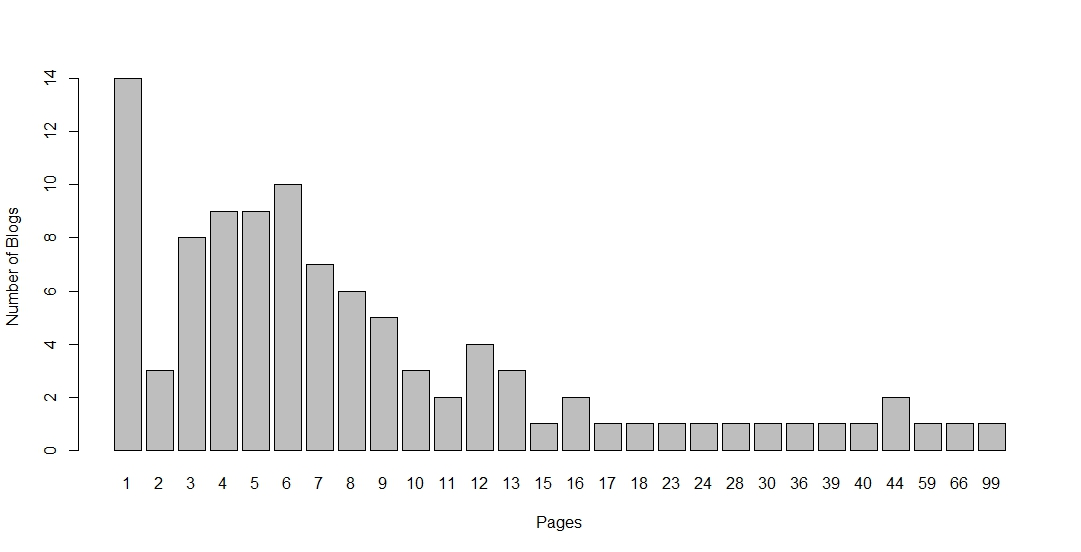
\includegraphics[width=1.2\textwidth]{hist}
\caption{Pages vs Number of Blogs}
\label{fig:hist}
\end{figure}

\lstset{
    language=R,
    caption={Pages vs Number of Blogs R},
     label=code:hist
}

\lstinputlisting{a9.r}

\section{Dendrograms}
Create an ASCII and JPEG dendrogram that clusters (i.e., HAC) the most similar blogs (see slides 12 \& 13).  
Include the JPEG in your report and upload the ascii file to github (it will be too unwieldy for inclusion in the report).

\subsection{Solution}
First I tried to change the provided function to output to a text file, but it was not successful.
So I redirected the standard output temporarily to blog\_ascii.txt, which is included with this report. \cite{bib:pystdout}
The JPEG dendogram was successful, as shown in Figure \ref{fig:jpeg}.  
The python code used is shown in Listing \ref{code:dendro}.\\

\lstset{
    caption={Create Dendrograms},
     label=code:dendro
}
\lstinputlisting[language=Python, firstline=202, lastline=209]{feedParse.py}

\begin{figure}[H]
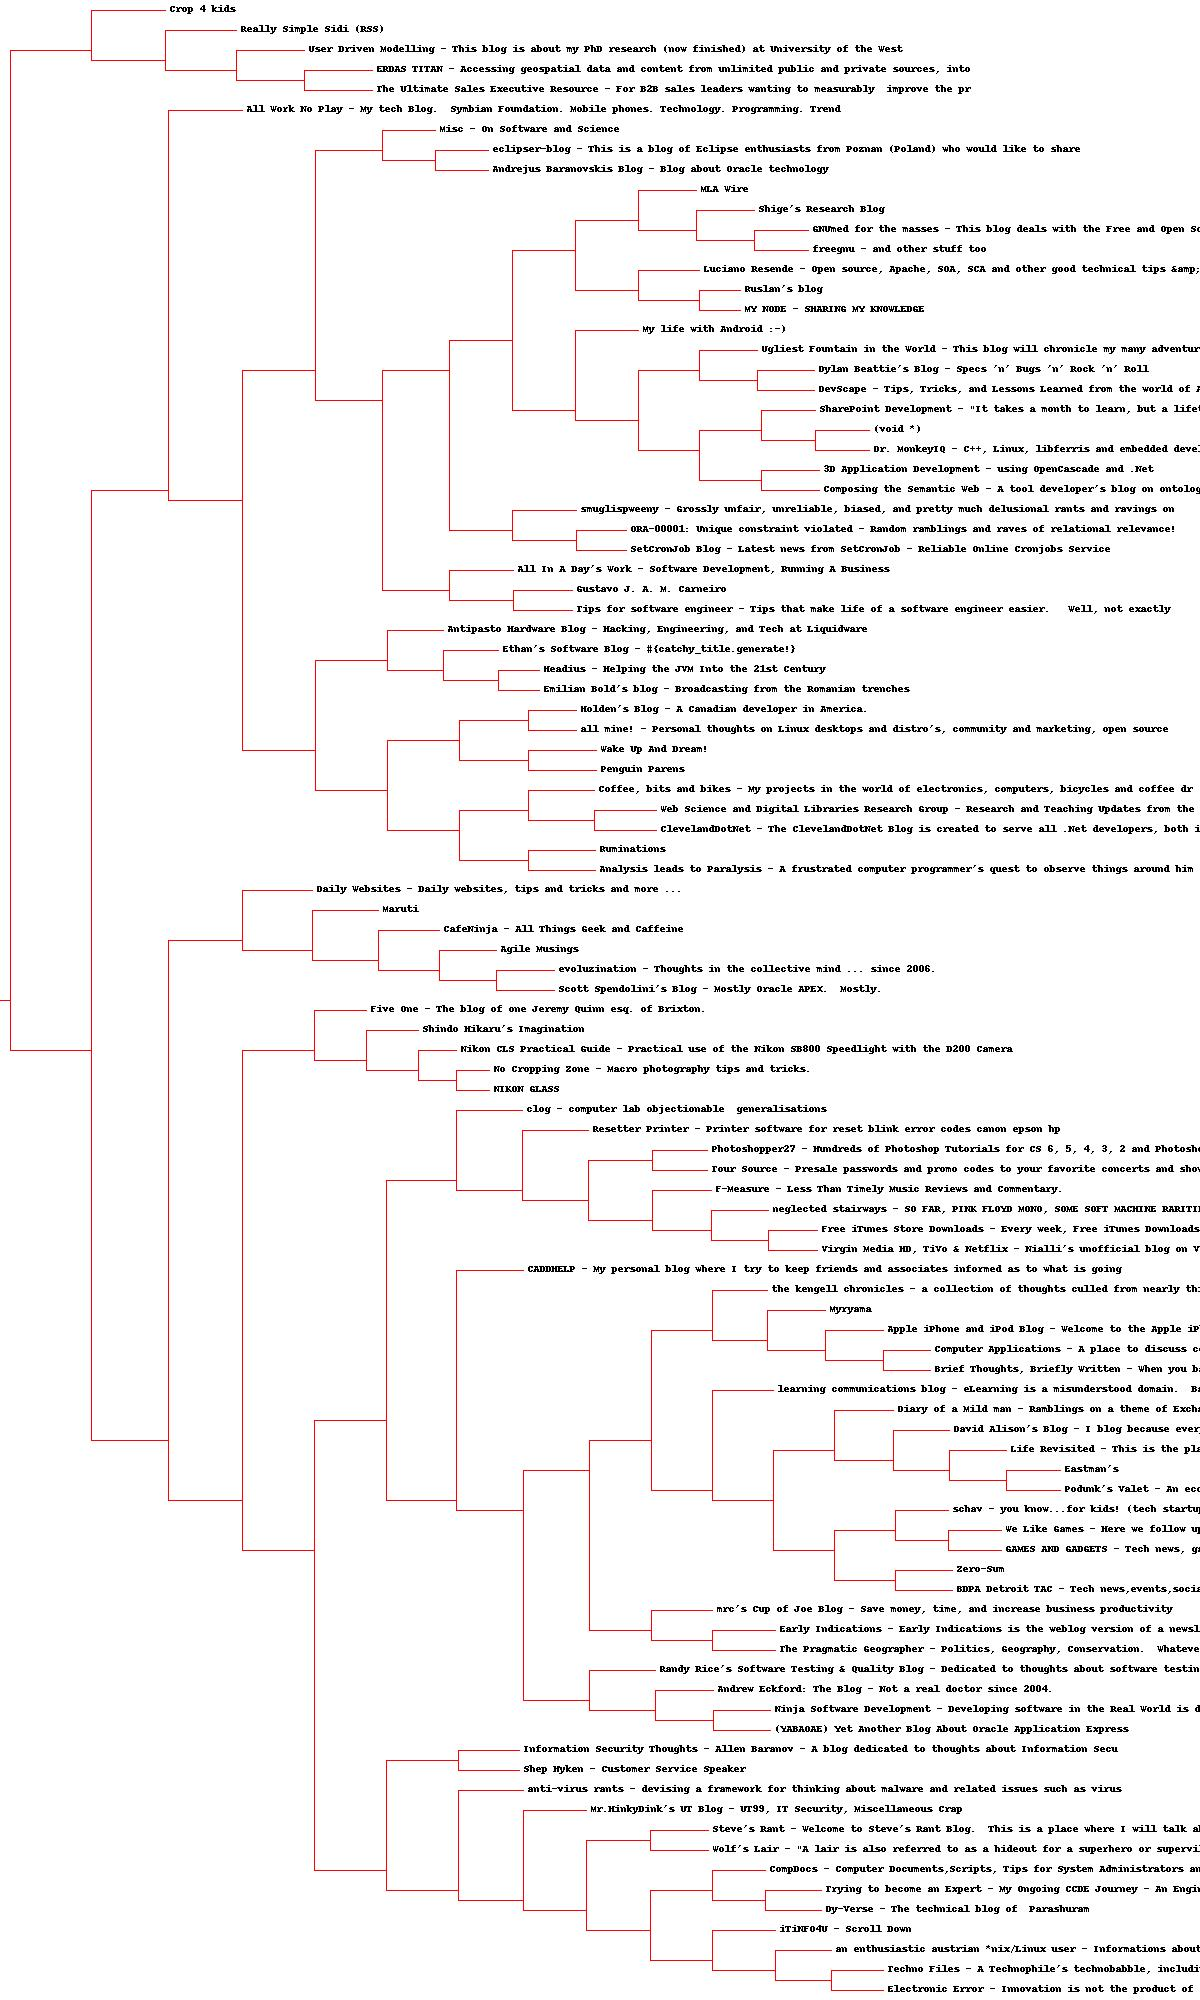
\includegraphics[width=1\textwidth]{output/blogclust}
\caption{jPEG Dendogram}
\label{fig:jpeg}
\end{figure}

\section{K-clustering}
Cluster the blogs using K-Means, using k=5,10,20. (see slide 18).
How many interations were required for each value of k?
\subsection{Solution}
To get the k-clustering, I used the provided functions in clusters.py from the PCI textbook, however, 
I also printed the resulting cluster to a file, blog\_k.txt.
For K = 5, the code took three iterations, but when K = 10 and 20, it took four iterations.
With five clusters, there was a group of `tips and tricks` blogs, three groups of technology blogs, for gadgets and software development, and a group of hobbies - photoshop, photography, concerts, etc.
When K was larger, the technology blogs were split up into smaller clusters, while the other clusters seemed to have stuck together.
The python code used to accomplish this is in Listing \ref{code:kclust}
The screen output from the code was saved as k\_run.txt\\

\lstset{
    caption={Create K-clusters},
     label=code:kclust
}
\lstinputlisting[language=Python, firstline=211, lastline=228]{feedParse.py}

\section{MDS}
Use MDS to create a JPEG of the blogs similar to slide 29.  
How many iterations were required?

\subsection{Solution}
In order to create the JPEG, the provided code from the PCI textbook was used.
The code used is shown in Listing \ref{code:mds}
This section took 265 iterations.
Although it wasn't required, the iteration numbers were saved as mds.txt, which also made it easier to count the iterations.\\

\lstset{
    caption={Create MDS},
     label=code:mds
}
\lstinputlisting[language=Python, firstline=202, lastline=209]{feedParse.py}

\begin{figure}[H]
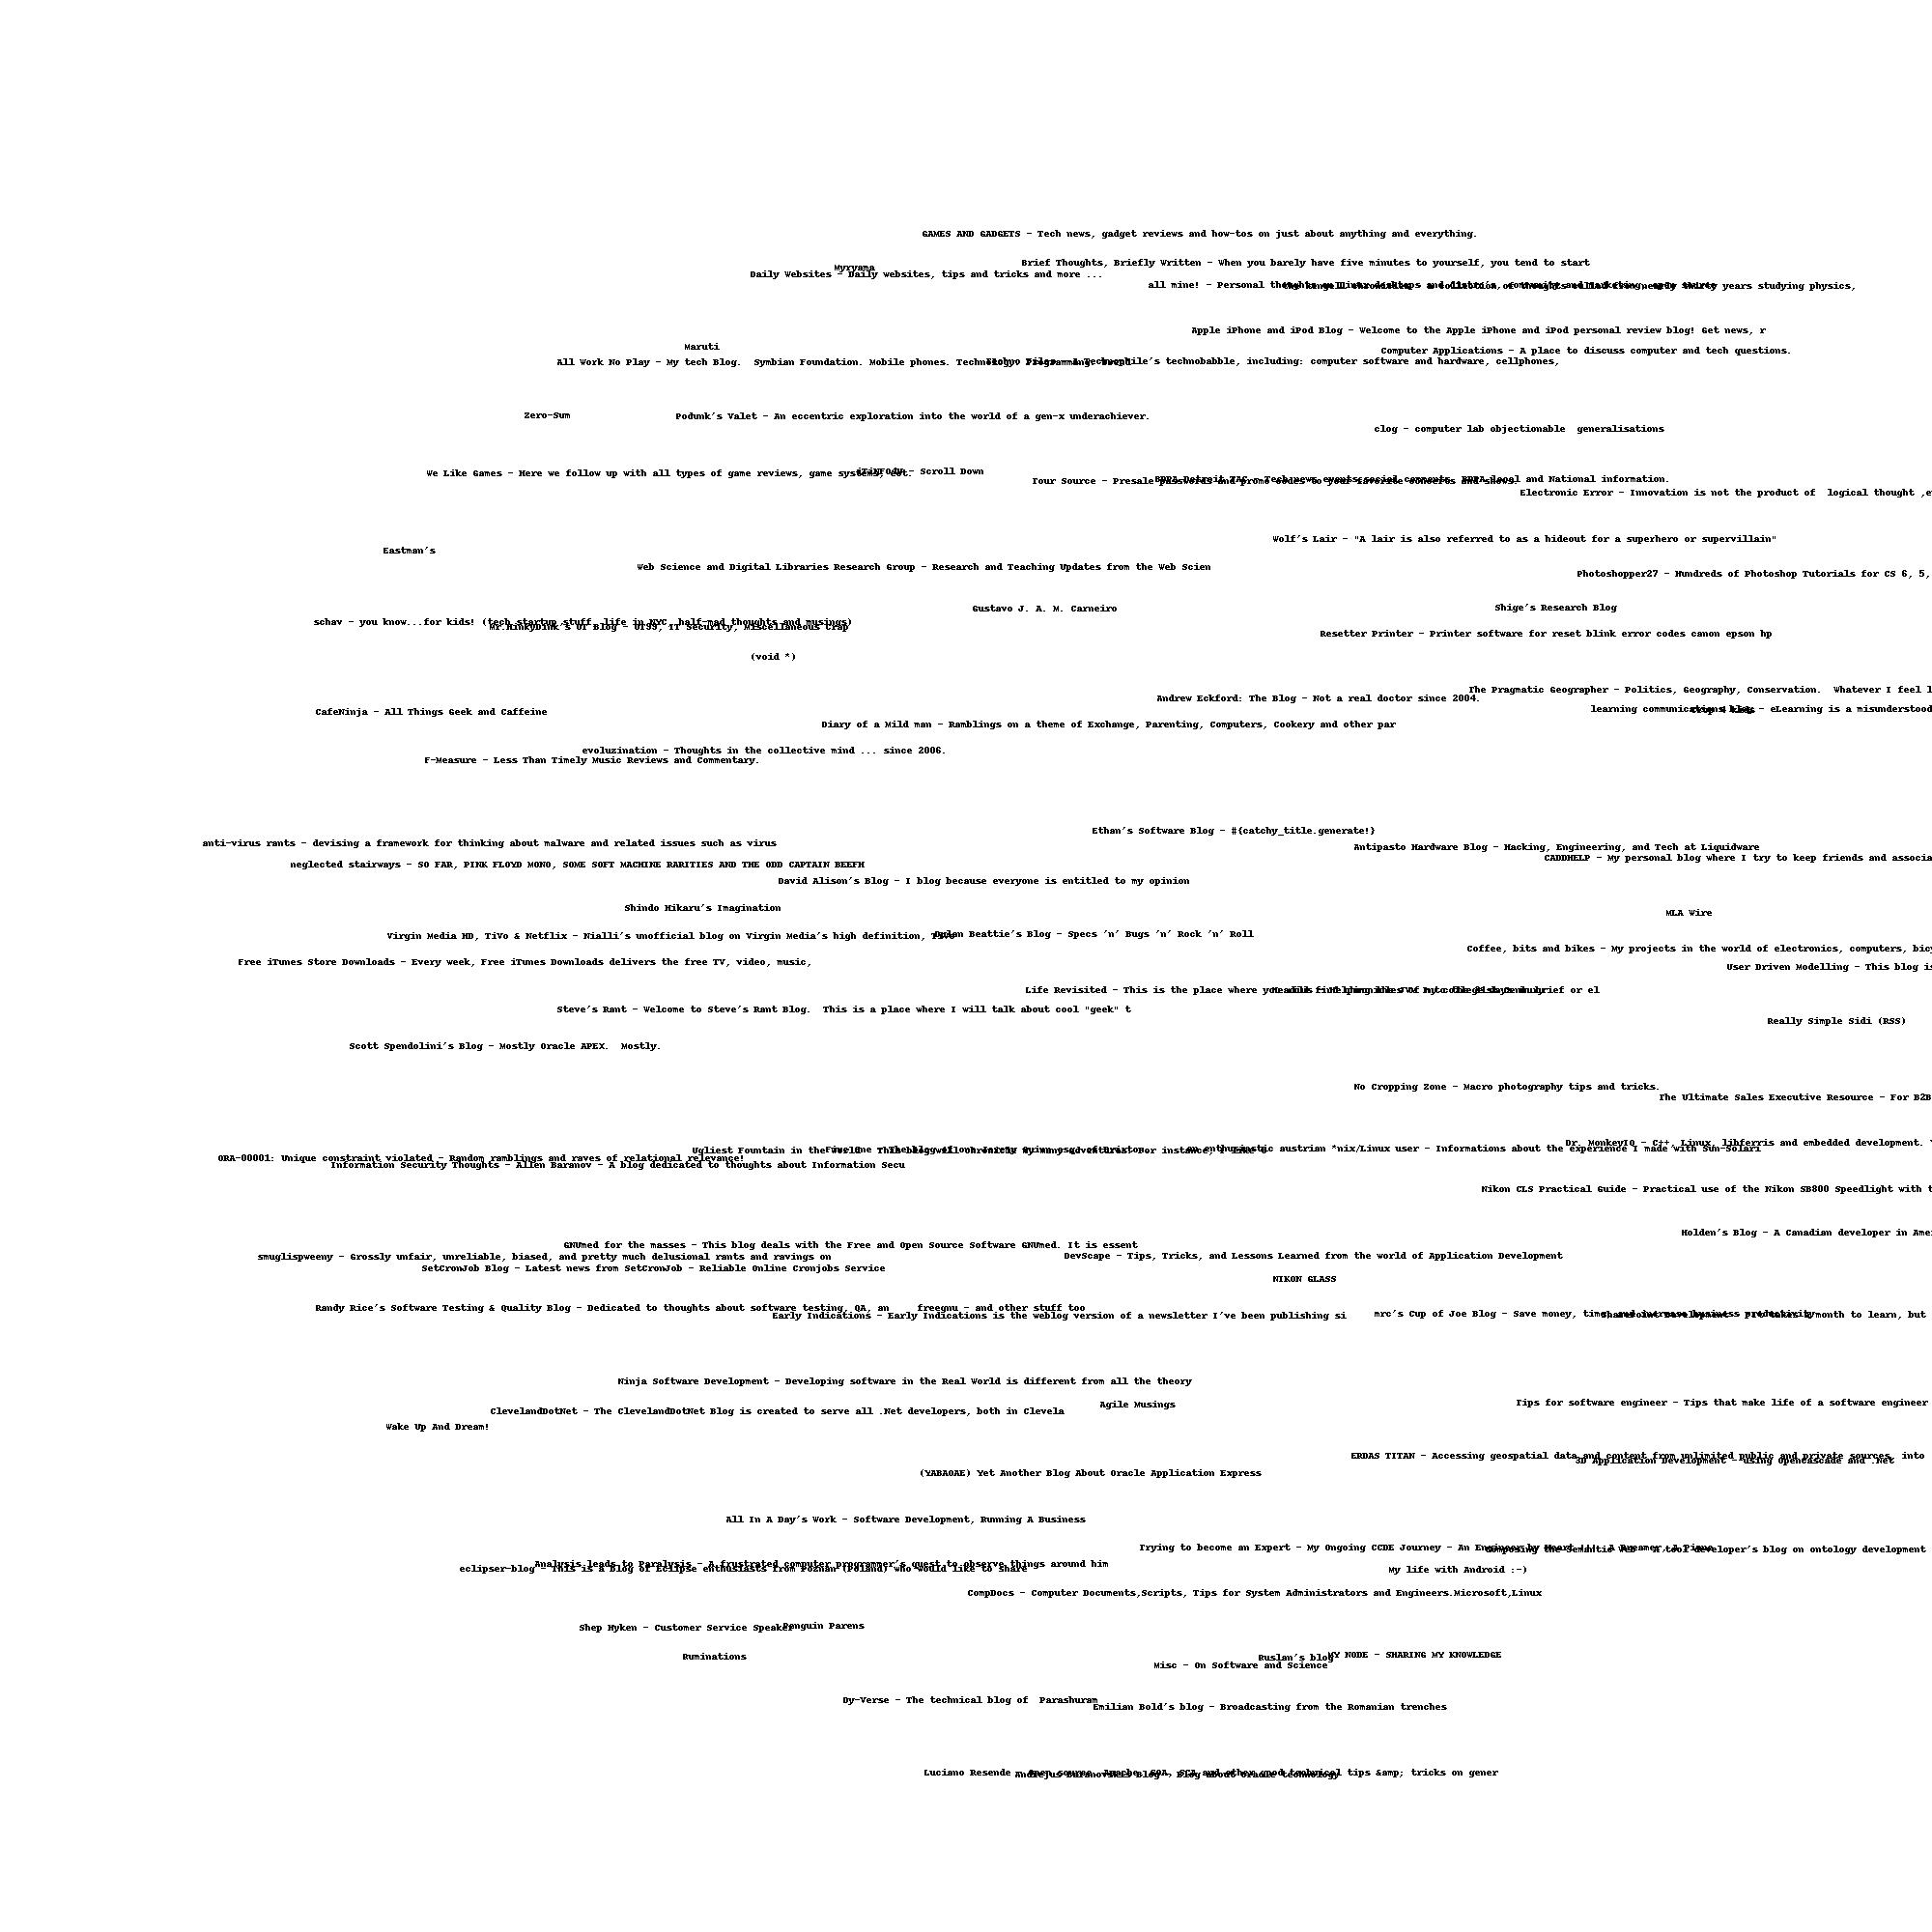
\includegraphics[width=1.2\textwidth]{output/blogs2d}
\caption{MDS}
\label{fig:mds}
\end{figure}

\newpage
\section{TFIDF}
Re-run question 2, but this time with proper TFIDF calculations instead of the hack discussed on slide 7 (p. 32).  
Use the same 500 words, but this time replace their frequency count with TFIDF scores as computed in assignment \#3.  
Document the code, techniques, methods, etc. used to generate these TFIDF values.  
Upload the new data file to github.
Compare and contrast the resulting dendrogram with the dendrogram
from question \#2.
\begin{description}
 \item[Note] ideally you would not reuse the same 500 terms and instead come up with TFIDF scores for all the terms and then choose the top 500 from that list, but I'm trying to limit the amount of work necessary.
\end{description}

\subsection{Solution}
TF is calculated as the word frequency divided by the total words in the document.
The IDF for each term was calculated as:
\[
IDF(\textrm{term})  = log_2(\textrm{total docs in corpus} / \textrm{docs with term})
\]
The total documents in corpus was used as the same as in Assignment Three, which was 42 billion.
In order to get the total documents with the term, the python module requests was used to perform the Google search.
Beautiful soup found the resultStats, which is where the number of results is stored.
My first run was caught by Google's bot detection, so I added a random number sleep element.
This took the program a little longer to run, but I was able to get all of the data.
The IDF for each term was saved in a dictionary keyed on the term, in order to calculate the TFIDF.

Another blog matrix was created and saved as blog\_tfidf.txt.
For each word, the TF was calculated using the count from the wordcount dictionary for the term, which was by blog, multiplied by the length of the wordcount entry for the blog, which was the total number of words in the blog.
Then TFIDF could be calculated as TF multiplied by IDF, and was rounded to three decimal points. \cite{bib:pyfunctions}

The last step was to create the new dendrograms.
It was similar to the previous dendrogram, if the blogs were not exactly next to each other after the TFIDF calculation, they were in close proximity.
This tells me that the ``hack'' provided by the book was a pretty good estimation for the TFIDF for each blog.
Figure \ref{fig:tfidf} is the new JPEG dendrogram.
Listing \ref{code:tfidf} is the python code used to accomplish this task.

\lstset{
    caption={TFIDF Calculation},
     label=code:tfidf
}
\lstinputlisting[language=Python, firstline=235, lastline=286]{feedParse.py}

\begin{figure}[H]
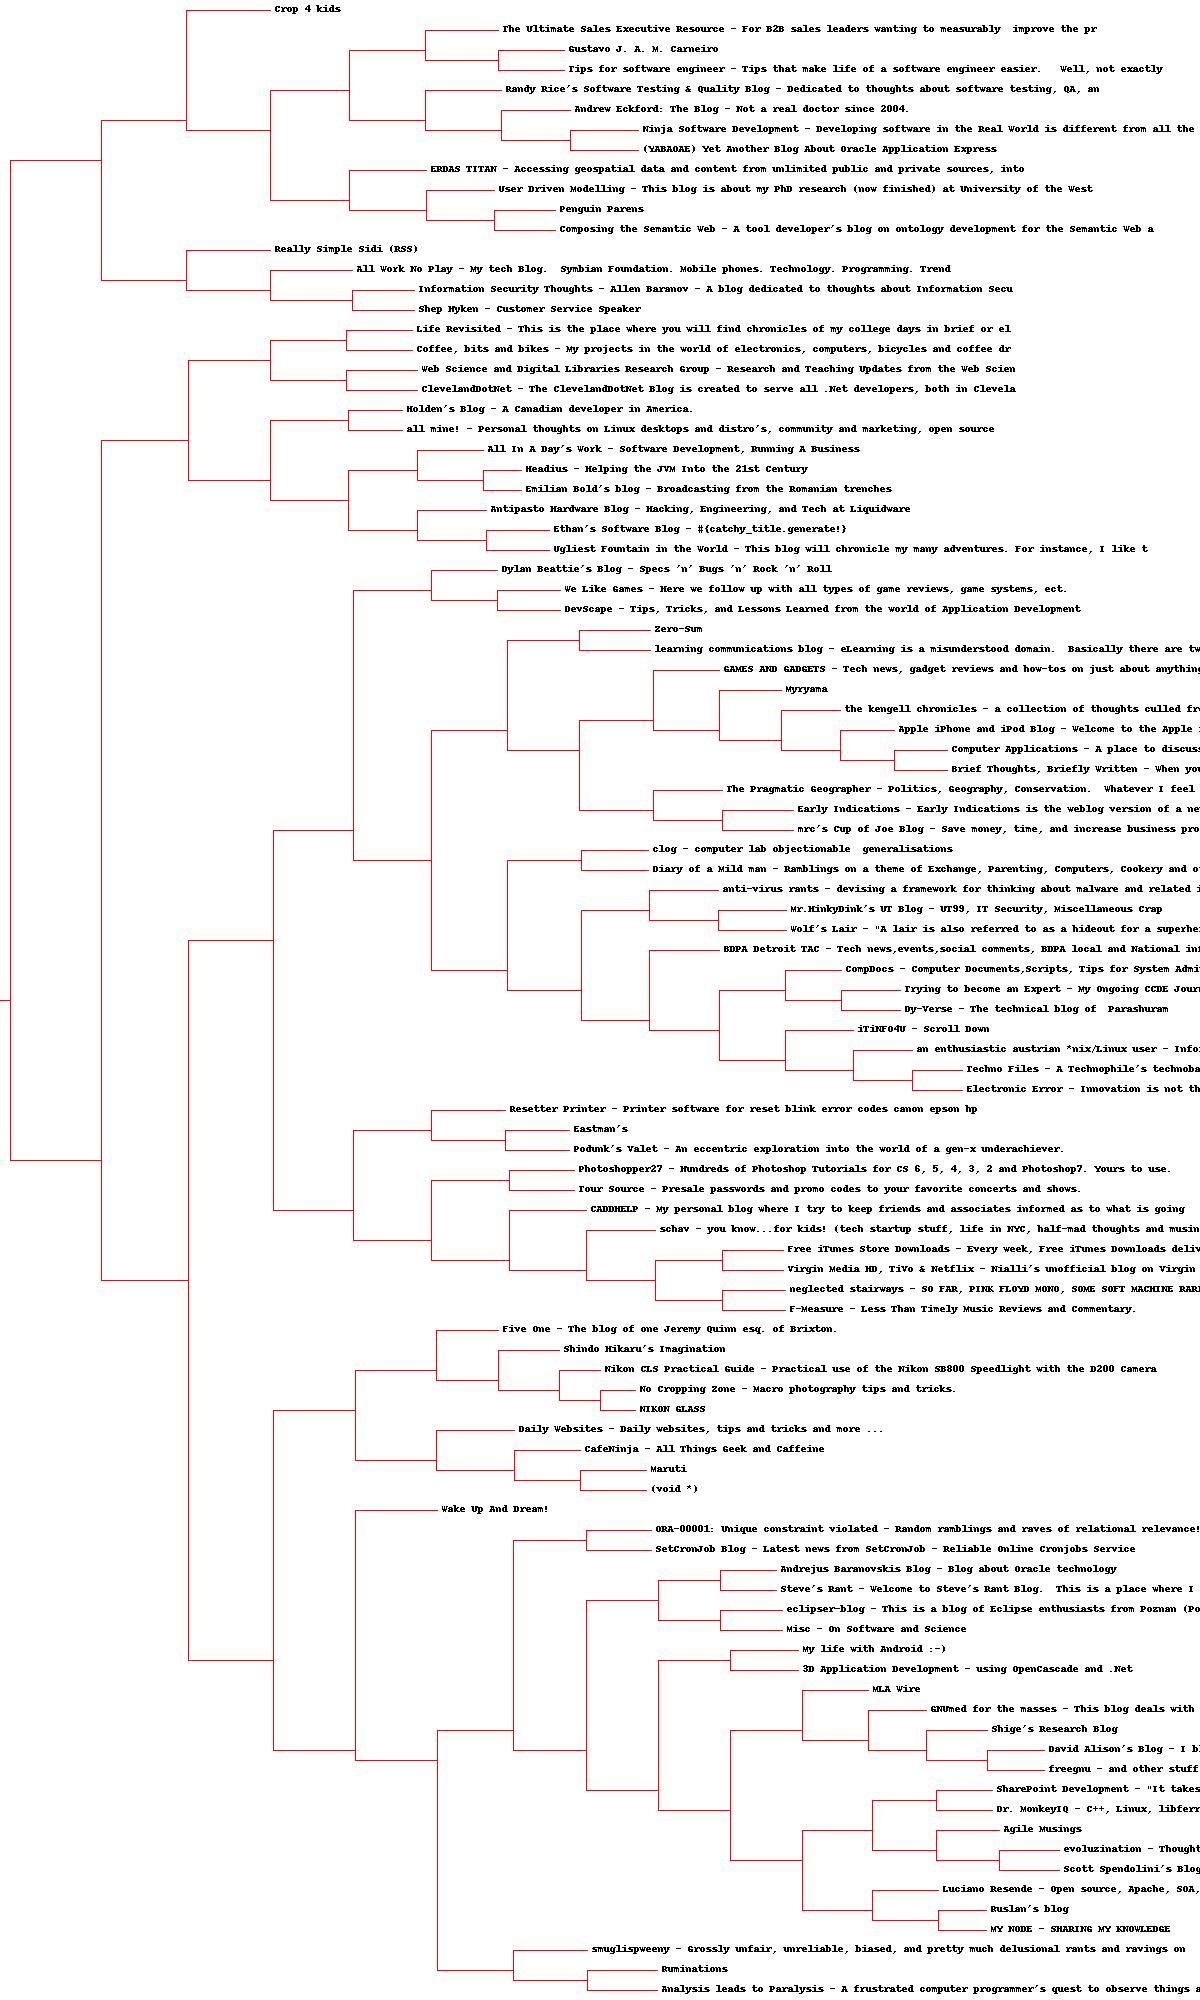
\includegraphics[width=1\textwidth]{output/tfidfclust}
\caption{TFIDF JPEG Dendogram}
\label{fig:tfidf}
\end{figure}

\newpage
\section{Python Code}
\label{sec:rec-code}
%%% Code Listing%%%%%

\lstset{
    language=python,
    caption={Complete Feed Parser},
     label=code:feedparse
}

\lstinputlisting{feedParse.py}
\newpage 


\bibliography{references}{}
\bibliographystyle{plain}
\end{document}